\chapter{Perancangan Block Cipher}
\label{ch:perancangan}

\section{Spesifikasi Umum}
\algname{} adalah \textit{block cipher} kunci simetris dengan spesifikasi seperti pada \cref{tab:spesifikasi}. Notasi yang dipakai di seluruh bab ini dirangkum pada \cref{tab:notasi}.

\begin{table}[H]
    \centering
    \caption{Spesifikasi \algname}
    \label{tab:spesifikasi}
    \begin{tabularx}{0.9\textwidth}{l Y}
        \toprule
        \textbf{Parameter} & \textbf{Nilai} \\
        \midrule
        Ukuran blok & 256 bit (32 byte), dibagi menjadi dua paruh 128 bit \\
        Panjang kunci & minimal 256 bit (32 byte); kunci di-\textit{hash} dengan SHA-256 menjadi 256 bit \\
        \textit{Nonce} & 256 bit (32 byte) acak dari CSPRNG, dibangkitkan setiap enkripsi \\
        Struktur & Jaringan Feistel 18 ronde \\
        Fungsi ronde & $f_{\text{GoL}}$ pada ronde 1 dan 18, $f_{\text{SPN}}$ pada ronde 2--17 \\
        \textit{Round key} & 18 buah, masing-masing 128 bit \\
        Penjadwalan kunci & SHA-256, lalu Game of Life $16 \times 16$ toroidal, 4 generasi per ronde, dengan injeksi ulang \textit{nonce} dan \textit{whitening} \\
        Mode operasi & ECB, CBC (bawaan), CFB, OFB, CTR \\
        \textit{Padding} & PKCS\#7 dengan ukuran blok 32 byte \\
        Keluaran & Base64$(\text{\textit{nonce}} \,\Vert\, C)$ \\
        \bottomrule
    \end{tabularx}
\end{table}

\begin{table}[H]
    \centering
    \caption{Notasi}
    \label{tab:notasi}
    \begin{tabularx}{0.9\textwidth}{l Y}
        \toprule
        \textbf{Notasi} & \textbf{Arti} \\
        \midrule
        $\oplus$ & XOR bit demi bit \\
        $\boxplus$ & penjumlahan per byte modulo 256 \\
        $x \rotl n$ & rotasi kiri $x$ sejauh $n$ bit \\
        $a \,\Vert\, b$ & penyambungan (konkatenasi) $a$ dan $b$ \\
        $L_i, R_i$ & paruh kiri dan kanan (masing-masing 128 bit) setelah ronde ke-$i$ \\
        $K_i$ & \textit{round key} ke-$i$ (128 bit), $1 \le i \le 18$ \\
        $N$ & \textit{nonce} 32 byte \\
        $\mathrm{GoL}^g(G)$ & hasil evolusi grid $G$ sebanyak $g$ generasi Game of Life \\
        \bottomrule
    \end{tabularx}
\end{table}

\section{Alur Global Enkripsi dan Dekripsi}
\Cref{fig:alur-global} memperlihatkan alur lengkap enkripsi sebuah pesan. Langkah-langkahnya adalah sebagai berikut.
\begin{enumerate}
    \item Kunci divalidasi (minimal 32 byte) dan data dikonversi menjadi \textit{bytes}.
    \item Data diberi \textit{padding} PKCS\#7 hingga panjangnya kelipatan 32 byte (\cref{sec:padding}).
    \item \textit{Nonce} 32 byte dibangkitkan secara acak.
    \item Penjadwalan kunci menurunkan 18 \textit{round key} dari kunci dan \textit{nonce} (\cref{sec:keysched}).
    \item Data dipotong menjadi blok 32 byte, lalu dienkripsi sesuai mode operasi (\cref{sec:mode}). Setiap pemanggilan $E$ menjalankan 18 ronde Feistel (\cref{sec:feistel}).
    \item \textit{Nonce} disambungkan di depan \textit{ciphertext}, lalu hasilnya dikodekan dengan Base64.
\end{enumerate}
Dekripsi menjalankan langkah sebaliknya: Base64 didekode, 32 byte pertama dibaca sebagai \textit{nonce}, \textit{round key} diturunkan ulang, setiap blok didekripsi sesuai mode, lalu \textit{padding} dibuang dan divalidasi.

\begin{figure}[H]
    \centering
    \begin{tikzpicture}[font=\small]
        \node[data] (pt) at (0,0) {\textit{Plaintext}\\(teks/biner)};
        \node[blok] (pad) at (2.55,0) {\textit{Padding}\\PKCS\#7};
        \node[blok] (split) at (4.75,0) {Potong blok\\32 byte};
        \node[blok, minimum width=3.6cm] (mode) at (8.3,0) {Mode operasi\\ECB/CBC/CFB/OFB/CTR};
        \node[blok] (b64) at (11.9,0) {Base64\\$(N \Vert C)$};

        \node[data] (key) at (0,-2) {Kunci $K$\\($\geq$ 32 byte)};
        \node[blokkunci] (ks) at (2.9,-2) {Penjadwalan\\kunci (GoL)};
        \node[blok, fill=red!8] (feistel) at (7.7,-2) {$E$: Feistel 18 ronde\\(\cref{fig:feistel})};
        \node[data] (nonce) at (2.9,-3.7) {\textit{Nonce} $N$ (32 byte acak)};

        \draw[panah] (pt) -- (pad);
        \draw[panah] (pad) -- (split);
        \draw[panah] (split) -- (mode);
        \draw[panah] (mode) -- (b64);
        \draw[panah] (key) -- (ks);
        \draw[panah] (nonce) -- (ks);
        \draw[panah] (ks) -- node[above, font=\scriptsize] {$K_1, \dots, K_{18}$} (feistel);
        \draw[panah, <->] (feistel.north) -- node[right, font=\scriptsize] {per blok} (feistel.north |- mode.south);
        \draw[panah] (nonce.east) -- (11.9,-3.7) -- node[pos=0.5, right, font=\scriptsize, align=left] {disisipkan\\di depan $C$} (b64.south);
        \fill (9.7,-3.7) circle (1.5pt);
        \draw[panah] (9.7,-3.7) -- node[pos=0.45, right, font=\scriptsize, align=left] {IV /\\\textit{counter}\\awal} ($(mode.south)+(1.4,0)$);
    \end{tikzpicture}
    \caption{Alur global enkripsi \algname}
    \label{fig:alur-global}
\end{figure}

\section{Jaringan Feistel 18 Ronde}
\label{sec:feistel}
Fungsi enkripsi satu blok $E$ memecah blok 256 bit $P$ menjadi $L_0 \Vert R_0$ (masing-masing 128 bit), lalu menjalankan 18 ronde Feistel:
\begin{equation}
    L_i = R_{i-1}, \qquad R_i = L_{i-1} \oplus F_i(R_{i-1}, K_i), \qquad
    F_i =
    \begin{cases}
        f_{\text{GoL}} & i \in \{1, 18\},\\
        f_{\text{SPN}} & 2 \le i \le 17.
    \end{cases}
    \label{eq:feistel-ps}
\end{equation}
Keluaran blok adalah $C = R_{18} \Vert L_{18}$, yaitu dengan pertukaran paruh terakhir dibatalkan seperti pada DES. Struktur ini diperlihatkan pada \cref{fig:feistel}.

Pemilihan fungsi ronde mengikuti peran masing-masing:
\begin{itemize}
    \item \textbf{Ronde 1 dan 18 ($f_{\text{GoL}}$)} berfungsi sebagai lapisan masuk dan keluar yang nonlinear dan berbeda sifat aljabarnya dari inti SPN. Penyerang yang ingin menganalisis inti SPN harus terlebih dahulu melewati transformasi GoL yang tidak memiliki deskripsi aljabar sederhana.
    \item \textbf{Ronde 2--17 ($f_{\text{SPN}}$)} memberikan jaminan \textit{confusion} dan \textit{diffusion} yang terukur melalui Kotak-S dan \code{MixColumns} AES.
\end{itemize}

\begin{figure}[H]
    \centering
    \begin{tikzpicture}[x=1cm, y=1cm, font=\small]
        \node[data, minimum width=7cm] (P) at (0,0) {Blok \textit{plaintext} $P$ (256 bit)};
        \node[data, minimum width=2.6cm] (L0) at (-2,-1.1) {$L_0$ (128 bit)};
        \node[data, minimum width=2.6cm] (R0) at (2,-1.1) {$R_0$ (128 bit)};
        \draw[panah] (P.south -| L0) -- (L0);
        \draw[panah] (P.south -| R0) -- (R0);

        % ronde 1
        \node[xorop] (x1) at (-2,-2.4) {};
        \node[blokgol, minimum width=2cm] (f1) at (0,-2.4) {$f_{\text{GoL}}$};
        \node (k1) at (0,-1.55) {$K_1$};
        \draw[panah] (L0) -- (x1);
        \draw[garis] (R0) -- (2,-2.4);
        \draw[panah] (2,-2.4) -- (f1);
        \draw[panah] (f1) -- (x1);
        \draw[panah] (k1) -- (f1);
        \draw[garis] (x1) -- (-2,-2.9) -- (2,-3.7);
        \draw[garis] (2,-2.4) -- (2,-2.9) -- (-2,-3.7);
        \node[left] at (-2,-3.9) {$L_1$};
        \node[right] at (2,-3.9) {$R_1$};

        % ronde 2
        \node[xorop] (x2) at (-2,-4.6) {};
        \node[blokspn, minimum width=2cm] (f2) at (0,-4.6) {$f_{\text{SPN}}$};
        \node (k2) at (0,-3.75) {$K_2$};
        \draw[panah] (-2,-3.7) -- (x2);
        \draw[garis] (2,-3.7) -- (2,-4.6);
        \draw[panah] (2,-4.6) -- (f2);
        \draw[panah] (f2) -- (x2);
        \draw[panah] (k2) -- (f2);
        \draw[garis] (x2) -- (-2,-5.1) -- (2,-5.9);
        \draw[garis] (2,-4.6) -- (2,-5.1) -- (-2,-5.9);
        \node[left] at (-2,-6.1) {$L_2$};
        \node[right] at (2,-6.1) {$R_2$};

        % ronde 3-17
        \draw[garis, dashed] (-2,-5.9) -- (-2,-7.1);
        \draw[garis, dashed] (2,-5.9) -- (2,-7.1);
        \node[blokspn, minimum width=3cm, fill=orange!7, dashed] at (0,-6.5) {ronde 3--17: $f_{\text{SPN}}$};
        \node[left] at (-2,-7.3) {$L_{17}$};
        \node[right] at (2,-7.3) {$R_{17}$};

        % ronde 18
        \node[xorop] (x18) at (-2,-8.1) {};
        \node[blokgol, minimum width=2cm] (f18) at (0,-8.1) {$f_{\text{GoL}}$};
        \node (k18) at (0,-7.25) {$K_{18}$};
        \draw[panah] (-2,-7.1) -- (x18);
        \draw[garis] (2,-7.1) -- (2,-8.1);
        \draw[panah] (2,-8.1) -- (f18);
        \draw[panah] (f18) -- (x18);
        \draw[panah] (k18) -- (f18);

        \node[data, minimum width=2.6cm] (R18) at (-2,-9.3) {$R_{18}$};
        \node[data, minimum width=2.6cm] (L18) at (2,-9.3) {$L_{18} = R_{17}$};
        \draw[panah] (x18) -- (R18);
        \draw[panah] (2,-8.1) -- (L18);
        \node[data, minimum width=7cm] (C) at (0,-10.5) {Blok \textit{ciphertext} $C = R_{18} \Vert L_{18}$ (256 bit)};
        \draw[panah] (R18) -- (R18 |- C.north);
        \draw[panah] (L18) -- (L18 |- C.north);

        \node[right, align=left, font=\scriptsize] at (3.8,-2.4) {\textcolor{green!45!black}{$\blacksquare$} ronde berbasis Game of Life};
        \node[right, align=left, font=\scriptsize] at (3.8,-4.6) {\textcolor{orange!80!black}{$\blacksquare$} ronde SPN gaya AES};
        \node[right, align=left, font=\scriptsize] at (3.8,-8.1) {ronde terakhir tanpa\\pertukaran paruh};
    \end{tikzpicture}
    \caption{Struktur jaringan Feistel 18 ronde pada \algname}
    \label{fig:feistel}
\end{figure}

\section{Fungsi Ronde \texorpdfstring{$f_{\text{GoL}}$}{f-GoL}}
\label{sec:fgol}
Fungsi ronde berbasis Game of Life didefinisikan sebagai
\begin{equation}
    f_{\text{GoL}}(R, K) = \mathrm{Ratakan}\big(\mathrm{GoL}^4(\mathrm{Grid}_{8\times16}(R \oplus K))\big) \oplus R.
    \label{eq:fgol}
\end{equation}
Langkah-langkahnya (\cref{fig:fgol}) adalah:
\begin{enumerate}
    \item \textbf{Pencampuran kunci.} $X = R \oplus K$ (128 bit).
    \item \textbf{Penyusunan grid.} 128 bit $X$ disusun menjadi grid 8 baris $\times$ 16 kolom secara \textit{big-endian}: dua byte pertama menjadi baris teratas, dan bit paling signifikan menjadi kolom paling kiri.
    \item \textbf{Evolusi.} Grid dievolusikan 4 generasi dengan aturan B3/S23 (\cref{eq:gol}) pada batas toroidal.
    \item \textbf{Perataan dan XOR umpan maju.} Grid hasil evolusi diratakan kembali menjadi 128 bit, lalu di-XOR dengan $R$.
\end{enumerate}

XOR umpan maju pada langkah terakhir penting karena evolusi GoL tidak injektif. Contoh ekstremnya, semua grid yang selnya mati atau terisolasi berevolusi menjadi grid kosong. Tanpa XOR dengan $R$, banyak nilai $R$ berbeda akan menghasilkan keluaran $F$ yang sama. Dengan XOR tersebut, dua masukan $R \neq R'$ yang tabrakan pada GoL tetap menghasilkan keluaran yang berbeda, karena selisihnya $R \oplus R'$ muncul langsung di keluaran.

\begin{figure}[H]
    \centering
    \begin{subfigure}[t]{0.47\textwidth}
        \centering
        \begin{tikzpicture}[node distance=0.45cm, font=\small]
            \node[data, minimum width=3.4cm] (in) {$R$ (128 bit)};
            \node[xorop, below=of in] (x) {};
            \node[left=0.5cm of x] (k) {$K_i$};
            \node[blokgol, below=of x, minimum width=3.6cm] (grid) {Susun grid $8 \times 16$ bit};
            \node[blokgol, below=of grid, minimum width=3.6cm] (gol) {$\mathrm{GoL}^4$: B3/S23, toroidal};
            \node[blokgol, below=of gol, minimum width=3.6cm] (flat) {Ratakan ke 128 bit};
            \node[xorop, below=of flat] (x2) {};
            \node[data, below=of x2, minimum width=3.4cm] (out) {$f_{\text{GoL}}(R, K_i)$};
            \draw[panah] (in) -- (x);
            \draw[panah] (k) -- (x);
            \draw[panah] (x) -- (grid);
            \draw[panah] (grid) -- (gol);
            \draw[panah] (gol) -- (flat);
            \draw[panah] (flat) -- (x2);
            \draw[panah] (x2) -- (out);
            \draw[panah] ($(in.south)+(1.2,0)$) -- ++(0,-0.2) -| ($(flat.east)+(0.45,0)$) |- (x2);
            \node[right, font=\scriptsize, align=left] at ($(gol.east)+(0.5,0)$) {umpan\\maju $R$};
        \end{tikzpicture}
        \caption{Fungsi ronde $f_{\text{GoL}}$ (ronde 1 dan 18)}
        \label{fig:fgol}
    \end{subfigure}\hfill
    \begin{subfigure}[t]{0.47\textwidth}
        \centering
        \begin{tikzpicture}[node distance=0.45cm, font=\small]
            \node[data, minimum width=3.4cm] (in) {$R$ (128 bit)};
            \node[xorop, below=of in] (x) {};
            \node[left=0.5cm of x] (k) {$K_i$};
            \node[blokspn, below=of x, minimum width=3.6cm] (sb) {\code{SubBytes} (Kotak-S)};
            \node[blokspn, below=of sb, minimum width=3.6cm] (sr) {\code{ShiftRows}};
            \node[blokspn, below=of sr, minimum width=3.6cm] (mc) {\code{MixColumns}};
            \node[addop, below=of mc] (add) {};
            \node[left=0.5cm of add] (k2) {$K_i$};
            \node[blokspn, below=of add, minimum width=3.6cm] (rot) {$\rotl \rho(Y)$ (128 bit)};
            \node[data, below=of rot, minimum width=3.4cm] (out) {$f_{\text{SPN}}(R, K_i)$};
            \draw[panah] (in) -- (x);
            \draw[panah] (k) -- (x);
            \draw[panah] (x) -- node[right, font=\scriptsize] {$X$} (sb);
            \draw[panah] (sb) -- (sr);
            \draw[panah] (sr) -- (mc);
            \draw[panah] (mc) -- (add);
            \draw[panah] (k2) -- (add);
            \draw[panah] (add) -- node[right, font=\scriptsize] {$Y$} (rot);
            \draw[panah] (rot) -- (out);
        \end{tikzpicture}
        \caption{Fungsi ronde $f_{\text{SPN}}$ (ronde 2--17)}
        \label{fig:fspn}
    \end{subfigure}
    \caption{Dua jenis fungsi ronde pada \algname}
    \label{fig:fungsi-ronde}
\end{figure}

\subsection{Implementasi Game of Life Secara Bit-Paralel}
Setiap baris grid disimpan sebagai satu bilangan bulat (\textit{bitmask}), sehingga satu generasi GoL dihitung per baris dengan operasi bitwise, bukan per sel. Untuk baris $r$, delapan tetangga diperoleh dari baris di atas, baris itu sendiri, dan baris di bawahnya (indeks modulo jumlah baris), masing-masing dalam versi asli serta versi yang dirotasi satu bit ke kiri dan ke kanan. Rotasi ini mewujudkan batas toroidal pada arah horizontal.

Kedelapan \textit{bitmask} tetangga dijumlahkan secara paralel untuk 16 sel sekaligus menggunakan pohon penjumlah ala Wallace \cite{wallace1964} (\cref{fig:wallace}). Hasilnya berupa tiga \textit{bitmask}: $c_0$ (bit ke-0 jumlah tetangga), $c_1$ (bit ke-1), dan $c_{\ge4}$ (jumlah tetangga $\geq 4$). Aturan B3/S23 kemudian cukup dihitung dengan
\begin{equation}
    s' = \underbrace{(c_1 \wedge \lnot c_{\ge 4})}_{N \in \{2,3\}} \wedge (c_0 \vee s),
\end{equation}
yang secara aljabar sama dengan $(N = 3) \vee (s \wedge N \in \{2,3\})$.

\begin{figure}[H]
    \centering
    \begin{tikzpicture}[font=\small, every node/.style={inner sep=2pt},
        fa/.style={rectangle, draw, fill=green!12, minimum width=0.9cm, minimum height=0.6cm},
        ha/.style={rectangle, draw, fill=green!5, minimum width=0.9cm, minimum height=0.6cm}]
        \foreach \i/\n in {0/{nw},1/n,2/{ne},3/w,4/e,5/{sw},6/s,7/{se}} {
            \node (n\i) at (\i*1.05, 0) {$n_{\n}$};
        }
        \node[fa] (fa1) at (1.05,-1.2) {FA};
        \node[fa] (fa2) at (4.2,-1.2) {FA};
        \node[ha] (ha1) at (6.82,-1.2) {HA};
        \foreach \i in {0,1,2} \draw[-Stealth] (n\i.south) -- (fa1.north);
        \foreach \i in {3,4,5} \draw[-Stealth] (n\i.south) -- (fa2.north);
        \foreach \i in {6,7} \draw[-Stealth] (n\i.south) -- (ha1.north);

        \node[fa] (fa3) at (2.2,-2.6) {FA};
        \node[fa] (fa4) at (5.5,-2.6) {FA};
        \draw[-Stealth] (fa1.south) -- (fa3.north);
        \draw[-Stealth] (fa2.south) -- (fa3.north);
        \draw[-Stealth] (ha1.south west) -- (fa3.north east);
        \draw[-Stealth, dashed] (fa1.south east) -- (fa4.north west);
        \draw[-Stealth, dashed] (fa2.south east) -- (fa4.north);
        \draw[-Stealth, dashed] (ha1.south) -- (fa4.north east);

        \node[ha] (ha2) at (4.0,-3.9) {HA};
        \draw[-Stealth, dashed] (fa3.south east) -- (ha2.north west);
        \draw[-Stealth] (fa4.south) -- (ha2.north east);

        \node[draw, rounded corners, fill=gray!8] (c0) at (1.0,-5.1) {$c_0$ (bobot 1)};
        \node[draw, rounded corners, fill=gray!8] (c1) at (4.0,-5.1) {$c_1$ (bobot 2)};
        \node[circle, draw, inner sep=1pt, font=\scriptsize] (or) at (6.9,-4.0) {OR};
        \node[draw, rounded corners, fill=gray!8] (c4) at (6.9,-5.1) {$c_{\ge4}$};
        \draw[-Stealth] (fa3.south) -- (c0.north);
        \draw[-Stealth] (ha2.south) -- (c1.north);
        \draw[-Stealth, dashed] (fa4.south east) -- (or.north);
        \draw[-Stealth, dashed] (ha2.east) -- (or.west);
        \draw[-Stealth] (or.south) -- (c4.north);
    \end{tikzpicture}
    \caption{Pohon penjumlah untuk menghitung jumlah tetangga 16 sel sekaligus (FA = \textit{full adder}, HA = \textit{half adder}; garis putus-putus = \textit{carry})}
    \label{fig:wallace}
\end{figure}

\section{Fungsi Ronde \texorpdfstring{$f_{\text{SPN}}$}{f-SPN}}
\label{sec:fspn}
Fungsi ronde SPN didefinisikan sebagai
\begin{align}
    X &= R \oplus K, \nonumber\\
    Y &= \mathrm{MixColumns}\big(\mathrm{ShiftRows}(\mathrm{SubBytes}(X))\big) \boxplus K, \label{eq:fspn}\\
    f_{\text{SPN}}(R, K) &= Y \rotl \rho(Y), \qquad \rho(Y) = \big((5 \cdot y_0 + y_{15}) \oplus y_8\big) \bmod 128, \nonumber
\end{align}
dengan $y_j$ byte ke-$j$ dari $Y$ dan rotasi dilakukan pada $Y$ sebagai bilangan 128 bit \textit{big-endian}. Alurnya ditunjukkan pada \cref{fig:fspn}.

\subsection{Susunan State}
Sebanyak 16 byte $X = x_0 x_1 \dots x_{15}$ disusun menjadi matriks $4 \times 4$ \textbf{baris demi baris}. Susunan ini berbeda dengan AES yang mengisi \textit{state} kolom demi kolom. Akibatnya, \code{ShiftRows} menggeser byte yang berurutan di dalam masukan, sedangkan \code{MixColumns} mencampur byte yang berjarak 4 posisi (lihat \cref{tab:shiftrows}).

\subsection{Kotak-S (SubBytes)}
Setiap byte disubstitusi dengan Kotak-S AES (\cref{tab:sbox}). Kotak-S ini dipilih setelah iterasi desain. Versi awal rancangan kami menggunakan Kotak-S afin $S(x) = (167x + 91) \bmod 256$, tetapi analisis pada \cref{sec:iterasi-sbox} menunjukkan bahwa Kotak-S afin meloloskan selisih \code{0x80} dengan peluang 1. Kotak-S AES memiliki keseragaman diferensial 4 dan bias linear maksimum 16/256. Kedua nilai ini merupakan yang terbaik yang diketahui untuk permutasi 8 bit.

\begin{table}[H]
    \centering
    \caption{Kotak-S $8 \times 8$ bit yang dipakai pada $f_{\text{SPN}}$ (nilai heksadesimal; baris = 4 bit atas, kolom = 4 bit bawah masukan)}
    \label{tab:sbox}
    \footnotesize
    \setlength{\tabcolsep}{4.2pt}
    \ttfamily
    \begin{tabular}{c|cccccccccccccccc}
        \toprule
        & \textbf{0} & \textbf{1} & \textbf{2} & \textbf{3} & \textbf{4} & \textbf{5} & \textbf{6} & \textbf{7} & \textbf{8} & \textbf{9} & \textbf{A} & \textbf{B} & \textbf{C} & \textbf{D} & \textbf{E} & \textbf{F} \\
        \midrule
        \textbf{0} & 63 & 7c & 77 & 7b & f2 & 6b & 6f & c5 & 30 & 01 & 67 & 2b & fe & d7 & ab & 76 \\
        \textbf{1} & ca & 82 & c9 & 7d & fa & 59 & 47 & f0 & ad & d4 & a2 & af & 9c & a4 & 72 & c0 \\
        \textbf{2} & b7 & fd & 93 & 26 & 36 & 3f & f7 & cc & 34 & a5 & e5 & f1 & 71 & d8 & 31 & 15 \\
        \textbf{3} & 04 & c7 & 23 & c3 & 18 & 96 & 05 & 9a & 07 & 12 & 80 & e2 & eb & 27 & b2 & 75 \\
        \textbf{4} & 09 & 83 & 2c & 1a & 1b & 6e & 5a & a0 & 52 & 3b & d6 & b3 & 29 & e3 & 2f & 84 \\
        \textbf{5} & 53 & d1 & 00 & ed & 20 & fc & b1 & 5b & 6a & cb & be & 39 & 4a & 4c & 58 & cf \\
        \textbf{6} & d0 & ef & aa & fb & 43 & 4d & 33 & 85 & 45 & f9 & 02 & 7f & 50 & 3c & 9f & a8 \\
        \textbf{7} & 51 & a3 & 40 & 8f & 92 & 9d & 38 & f5 & bc & b6 & da & 21 & 10 & ff & f3 & d2 \\
        \textbf{8} & cd & 0c & 13 & ec & 5f & 97 & 44 & 17 & c4 & a7 & 7e & 3d & 64 & 5d & 19 & 73 \\
        \textbf{9} & 60 & 81 & 4f & dc & 22 & 2a & 90 & 88 & 46 & ee & b8 & 14 & de & 5e & 0b & db \\
        \textbf{A} & e0 & 32 & 3a & 0a & 49 & 06 & 24 & 5c & c2 & d3 & ac & 62 & 91 & 95 & e4 & 79 \\
        \textbf{B} & e7 & c8 & 37 & 6d & 8d & d5 & 4e & a9 & 6c & 56 & f4 & ea & 65 & 7a & ae & 08 \\
        \textbf{C} & ba & 78 & 25 & 2e & 1c & a6 & b4 & c6 & e8 & dd & 74 & 1f & 4b & bd & 8b & 8a \\
        \textbf{D} & 70 & 3e & b5 & 66 & 48 & 03 & f6 & 0e & 61 & 35 & 57 & b9 & 86 & c1 & 1d & 9e \\
        \textbf{E} & e1 & f8 & 98 & 11 & 69 & d9 & 8e & 94 & 9b & 1e & 87 & e9 & ce & 55 & 28 & df \\
        \textbf{F} & 8c & a1 & 89 & 0d & bf & e6 & 42 & 68 & 41 & 99 & 2d & 0f & b0 & 54 & bb & 16 \\
        \bottomrule
    \end{tabular}
\end{table}


\subsection{ShiftRows dan MixColumns}
\code{ShiftRows} merotasi baris ke-$i$ ($i = 0,1,2,3$) ke kiri sejauh $i$ byte (\cref{tab:shiftrows}). \code{MixColumns} mengalikan setiap kolom $(a_0, a_1, a_2, a_3)^T$ dengan matriks MDS AES di GF($2^8$):
\begin{equation}
    \begin{bmatrix} b_0 \\ b_1 \\ b_2 \\ b_3 \end{bmatrix} =
    \begin{bmatrix} 02 & 03 & 01 & 01 \\ 01 & 02 & 03 & 01 \\ 01 & 01 & 02 & 03 \\ 03 & 01 & 01 & 02 \end{bmatrix}
    \begin{bmatrix} a_0 \\ a_1 \\ a_2 \\ a_3 \end{bmatrix},
\end{equation}
dengan perkalian $02 \cdot a = (a \ll 1) \oplus (\texttt{0x1B} \text{ jika bit 7 } a = 1)$ dan $03 \cdot a = (02 \cdot a) \oplus a$. Kedua tabel perkalian ini dihitung di awal sebagai tabel \textit{lookup}.

\begin{table}[H]
    \centering
    \caption{Susunan \textit{state} $4\times4$ sebelum dan sesudah \code{ShiftRows} (indeks byte masukan)}
    \label{tab:shiftrows}
    \begin{tabular}{cccc c cccc}
        \multicolumn{4}{c}{\textbf{Sebelum}} & \quad & \multicolumn{4}{c}{\textbf{Sesudah}} \\
        \cmidrule{1-4} \cmidrule{6-9}
        $x_0$ & $x_1$ & $x_2$ & $x_3$ & & $x_0$ & $x_1$ & $x_2$ & $x_3$ \\
        $x_4$ & $x_5$ & $x_6$ & $x_7$ & $\xrightarrow{\;\ll 1\;}$ & $x_5$ & $x_6$ & $x_7$ & $x_4$ \\
        $x_8$ & $x_9$ & $x_{10}$ & $x_{11}$ & $\xrightarrow{\;\ll 2\;}$ & $x_{10}$ & $x_{11}$ & $x_8$ & $x_9$ \\
        $x_{12}$ & $x_{13}$ & $x_{14}$ & $x_{15}$ & $\xrightarrow{\;\ll 3\;}$ & $x_{15}$ & $x_{12}$ & $x_{13}$ & $x_{14}$ \\
    \end{tabular}
\end{table}

\subsection{Penjumlahan Modular dan Rotasi Bergantung Data}
Setelah \code{MixColumns}, \textit{state} dijumlahkan dengan \textit{round key} per byte modulo 256 ($\boxplus$). Kunci dengan demikian masuk dua kali ke $f_{\text{SPN}}$ melalui dua operasi dari struktur aljabar yang berbeda: XOR (penjumlahan di GF(2)) dan penjumlahan bilangan bulat modulo 256. Pencampuran kedua operasi ini, seperti pada IDEA dan RC6 \cite{rivest1998}, mempersulit analisis yang hanya bekerja di satu struktur aljabar.

Langkah terakhir adalah rotasi kiri 128 bit sejauh $\rho(Y) \in [0, 127]$ yang dihitung dari tiga byte $Y$ sendiri. Ide ini diambil dari RC5/RC6. Karena besar rotasi bergantung pada data, penyerang tidak dapat memprediksi posisi bit keluaran tanpa mengetahui nilai antara. Rotasi juga memindahkan bit melintasi batas byte, sehingga melengkapi \code{MixColumns} yang hanya bekerja di dalam kolom.

\section{Penjadwalan Kunci (Round Key)}
\label{sec:keysched}
Penjadwalan kunci menurunkan 18 \textit{round key} 128 bit dari kunci $K$ dan \textit{nonce} $N$. Gagasan utamanya adalah menjadikan kunci sebagai konfigurasi awal Game of Life, lalu mengambil \textit{round key} dari hasil evolusinya setelah di-\textit{whitening}. Alur lengkapnya ditunjukkan pada \cref{fig:keysched}.

\begin{figure}[H]
    \centering
    \begin{tikzpicture}[node distance=0.42cm, font=\small]
        \node[data] (k) {Kunci $K$ ($\geq$ 32 byte)};
        \node[blokkunci, below=of k, minimum width=7.4cm] (fold) {(1) Validasi, lalu \textit{hash}: $k_0 \dots k_{31} = \mathrm{SHA\text{-}256}(K)$};
        \node[blokkunci, below=of fold, minimum width=7.4cm] (mix) {(2) Campur: $m_i = (k_i \rotl (n_i \bmod 8)) \oplus n_i$};
        \node[blokkunci, below=of mix, minimum width=7.4cm] (spiral) {(3) Isi spiral grid $16\times16$: sel ke-$j$ $= (m_{j \bmod 32} + 31\lfloor j/32 \rfloor) \bmod 256$};
        \node[blokkunci, below=of spiral, minimum width=7.4cm] (par) {(4) Paritas tiap sel $\Rightarrow$ pola biner $\mathrm{Pola}(K, N)$};
        \node[blok, below=0.55cm of par, minimum width=4cm] (g0) {$G \leftarrow \mathrm{Pola}(K, N)$};

        \node[blokgol, below=0.7cm of g0, minimum width=7.4cm] (reinj) {(5) $N_r = \mathrm{RotByte}(N, r) \oplus (17r \bmod 256)$;\; $P_r = \mathrm{Pola}(K, N_r)$;\; $G \leftarrow G \oplus P_r$};
        \node[blokgol, below=of reinj, minimum width=7.4cm] (evo) {(6) $G \leftarrow \mathrm{GoL}^4(G)$ pada grid $16 \times 16$ toroidal};
        \node[blokgol, below=of evo, minimum width=7.4cm] (rk) {(7) \textit{Whitening} $W = G \oplus P_r$;\; $K_r = W_{\text{baris }0\text{--}7} \oplus W_{\text{baris }8\text{--}15}$};
        \node[keputusan, below=0.5cm of rk] (cek) {$r < 18$?};
        \node[data, below=0.5cm of cek] (out) {$K_1, K_2, \dots, K_{18}$};

        \node[data, right=1.0cm of mix] (n) {\textit{Nonce} $N$};

        \draw[panah] (k) -- (fold);
        \draw[panah] (fold) -- (mix);
        \draw[panah] (mix) -- (spiral);
        \draw[panah] (spiral) -- (par);
        \draw[panah] (par) -- (g0);
        \draw[panah] (g0) -- node[right] {$r = 1$} (reinj);
        \draw[panah] (reinj) -- (evo);
        \draw[panah] (evo) -- (rk);
        \draw[panah] (rk) -- (cek);
        \draw[panah] (cek) -- node[right] {tidak} (out);
        \draw[panah] (cek.west) -- node[above] {ya} ($(cek.west -| reinj.west)+(-0.5,0)$) |- node[pos=0.25, left] {$r \leftarrow r+1$} (reinj.west);
        \draw[panah] (n) -- (mix);
        \draw[panah] (n.south) |- (reinj.east);

        \begin{scope}[on background layer]
            \node[draw, dashed, rounded corners, fill=violet!3, fit=(fold)(par), inner sep=5pt, label={[font=\scriptsize, anchor=south east]north east:fungsi $\mathrm{Pola}(K, N)$}] {};
        \end{scope}
    \end{tikzpicture}
    \caption{Alur penjadwalan kunci berbasis Game of Life}
    \label{fig:keysched}
\end{figure}

Rincian setiap langkahnya adalah sebagai berikut.
\begin{enumerate}
    \item \textbf{Validasi dan \textit{hashing}.} Kunci minimal 32 byte (256 bit). Kunci sepanjang apa pun di-\textit{hash} dengan SHA-256 menjadi 32 byte $k_0, \dots, k_{31}$, sehingga setiap byte kunci memengaruhi seluruh materi kunci dan tidak ada dua kunci berbeda yang (secara praktis) menghasilkan materi yang sama.
    \item \textbf{Pencampuran dengan \textit{nonce}.} Setiap byte kunci dirotasi kiri 8 bit sejauh $n_i \bmod 8$, lalu di-XOR dengan $n_i$ (byte \textit{nonce} ke-$i$). Untuk \textit{nonce} tetap, langkah ini merupakan bijeksi pada setiap byte.
    \item \textbf{Pengisian spiral.} Ke-32 byte $m_i$ diisikan ke grid $16 \times 16$ mengikuti spiral searah jarum jam dari pojok kiri atas ke pusat (\cref{fig:spiral}). Karena grid memiliki 256 sel, materi 32 byte berulang sebanyak 8 putaran. Pada putaran ke-$\ell$ ($\ell = 0, \dots, 7$), nilainya ditambah $31\ell$ modulo 256 agar setiap putaran tidak sekadar menyalin putaran sebelumnya.
    \item \textbf{Paritas.} Setiap sel diganti dengan paritas jumlah bit 1-nya ($\mathrm{popcount} \bmod 2$), sehingga diperoleh grid biner $16 \times 16$ (256 bit) dengan kepadatan sel hidup sekitar 0,5.
    \item \textbf{Injeksi ulang \textit{nonce}.} Pada ronde ke-$r$, \textit{nonce} dirotasi sejauh $r$ byte dan setiap byte-nya di-XOR dengan $17r \bmod 256$. Pola baru $\mathrm{Pola}(K, N_r)$ dihitung dengan langkah 1--4, lalu di-XOR ke grid. Injeksi ulang mencegah grid mati atau terjebak pada pola periodik (osilator atau \textit{still life}), sehingga setiap ronde menerima entropi baru dari kunci.
    \item \textbf{Evolusi.} Grid dievolusikan 4 generasi Game of Life pada grid toroidal $16 \times 16$.
    \item \textbf{\textit{Whitening} dan pelipatan.} Grid hasil evolusi di-XOR sekali lagi dengan pola injeksi $P_r$ dari langkah 5, menghasilkan $W = G \oplus P_r$. Grid 256 bit $W$ kemudian dilipat menjadi \textit{round key} 128 bit dengan meng-XOR-kan 8 baris atas dengan 8 baris bawah. Langkah \textit{whitening} ini menyeimbangkan proporsi bit 1 pada \textit{round key} (\cref{sec:rk-density}). Grid yang dibawa ke ronde berikutnya tetap $G$ (hasil evolusi tanpa \textit{whitening}).
\end{enumerate}

\begin{figure}[H]
    \centering
    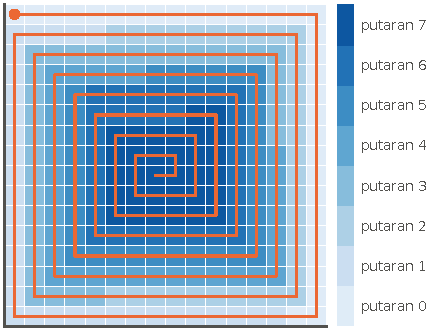
\includegraphics[width=0.42\textwidth]{spiral.pdf}
    \caption{Urutan pengisian spiral grid $16 \times 16$. Garis oranye menunjukkan urutan sel, dan warna menunjukkan putaran materi kunci ke-$\ell$ (32 sel per putaran).}
    \label{fig:spiral}
\end{figure}

\Cref{fig:ks-stages} menunjukkan contoh nyata tahapan penjadwalan kunci untuk kunci \code{"kunci-\allowbreak rahasia-\allowbreak minimal-\allowbreak 32-byte!!!"} dengan \textit{nonce} $N = \mathrm{SHA\text{-}256}(\texttt{"IF4020"})$. \textit{Round key} pertama yang dihasilkan adalah
\begin{center}
    $K_1 = $ \code{f9ec878321d2537857cb46413165e4f2}.
\end{center}

\begin{figure}[H]
    \centering
    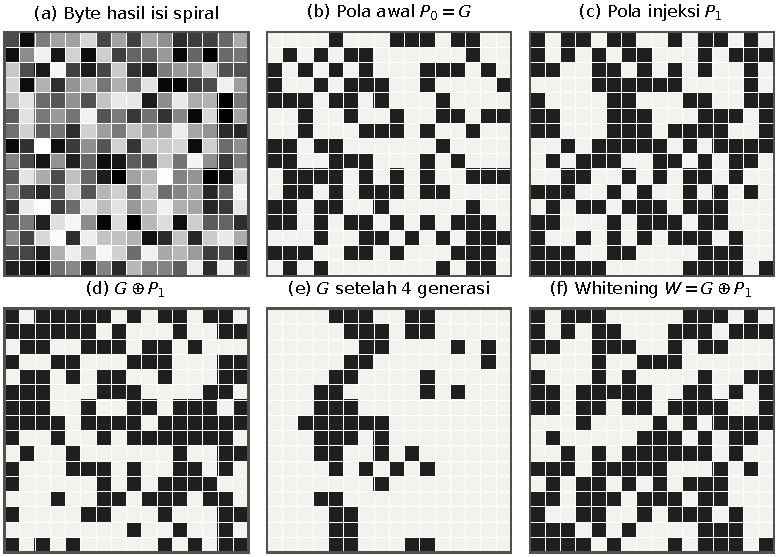
\includegraphics[width=0.86\textwidth]{ks_stages.pdf}
    \caption{Contoh tahapan penjadwalan kunci pada ronde pertama. Sel hitam bernilai 1 (hidup); panel (a) menampilkan nilai byte 0--255 dalam skala abu-abu. Panel (f) adalah grid yang dilipat menjadi $K_1$.}
    \label{fig:ks-stages}
\end{figure}

\section{Dekripsi}
\label{sec:dekripsi}
Karena memakai struktur Feistel, dekripsi blok menggunakan prosedur yang sama dengan enkripsi, tetapi \textit{round key} dipakai dengan urutan terbalik. Masukan $C$ dipecah menjadi $L'_0 \Vert R'_0 = R_{18} \Vert L_{18}$, lalu untuk $j = 1, \dots, 18$ dengan indeks kunci $i = 19 - j$:
\begin{equation}
    L'_j = R'_{j-1}, \qquad R'_j = L'_{j-1} \oplus F_i(R'_{j-1}, K_i).
\end{equation}
Jenis fungsi ronde mengikuti indeks kunci $i$, bukan urutan eksekusi $j$. Dengan demikian, ronde dekripsi pertama memakai $f_{\text{GoL}}$ dengan $K_{18}$, dan ronde terakhir memakai $f_{\text{GoL}}$ dengan $K_1$ (\cref{tab:urutan-dekripsi}). Kebenaran dekripsi dapat ditunjukkan dengan induksi. Pada ronde pertama, $R'_1 = R_{18} \oplus F_{18}(L_{18}, K_{18}) = R_{18} \oplus F_{18}(R_{17}, K_{18}) = L_{17}$ dan $L'_1 = R_{17}$. Pola yang sama berulang hingga $R'_{18} \Vert L'_{18}$ bernilai $L_0 \Vert R_0 = P$. Pembuktian ini tidak memerlukan $f_{\text{GoL}}$ maupun $f_{\text{SPN}}$ untuk dapat dibalik.

\begin{table}[H]
    \centering
    \caption{Urutan ronde pada enkripsi dan dekripsi}
    \label{tab:urutan-dekripsi}
    \begin{tabular}{c cc c cc}
        \toprule
        \multirow{2}{*}{\textbf{Urutan}} & \multicolumn{2}{c}{\textbf{Enkripsi}} & & \multicolumn{2}{c}{\textbf{Dekripsi}} \\
        \cmidrule{2-3} \cmidrule{5-6}
        & Kunci & Fungsi & & Kunci & Fungsi \\
        \midrule
        1 & $K_1$ & $f_{\text{GoL}}$ & & $K_{18}$ & $f_{\text{GoL}}$ \\
        2 & $K_2$ & $f_{\text{SPN}}$ & & $K_{17}$ & $f_{\text{SPN}}$ \\
        $\vdots$ & $\vdots$ & $\vdots$ & & $\vdots$ & $\vdots$ \\
        17 & $K_{17}$ & $f_{\text{SPN}}$ & & $K_2$ & $f_{\text{SPN}}$ \\
        18 & $K_{18}$ & $f_{\text{GoL}}$ & & $K_1$ & $f_{\text{GoL}}$ \\
        \bottomrule
    \end{tabular}
\end{table}

\section{Mode Operasi}
\label{sec:mode}
\algname{} mendukung lima mode operasi standar \cite{sp80038a} dengan ukuran blok penuh 256 bit (\cref{tab:mode}). \textit{Nonce} berperan ganda. Pada semua mode, \textit{nonce} dipakai dalam penjadwalan kunci. Pada mode selain ECB, \textit{nonce} juga menjadi IV atau nilai awal \textit{counter}. Pemakaian ganda ini aman karena \textit{nonce} dibangkitkan secara acak untuk setiap pesan, dan IV memang tidak perlu dirahasiakan.

\begin{table}[H]
    \centering
    \caption{Mode operasi yang didukung ($E$/$D$ = enkripsi/dekripsi satu blok, $C_0 = O_0 = N$)}
    \label{tab:mode}
    \small
    \begin{tabularx}{\textwidth}{l l l Y}
        \toprule
        \textbf{Mode} & \textbf{Enkripsi} & \textbf{Dekripsi} & \textbf{Keterangan} \\
        \midrule
        ECB & $C_i = E(P_i)$ & $P_i = D(C_i)$ & Blok identik dalam satu pesan menghasilkan \textit{ciphertext} identik \\
        CBC & $C_i = E(P_i \oplus C_{i-1})$ & $P_i = D(C_i) \oplus C_{i-1}$ & Mode bawaan \\
        CFB & $C_i = P_i \oplus E(C_{i-1})$ & $P_i = C_i \oplus E(C_{i-1})$ & CFB blok penuh (256 bit), hanya memakai $E$ \\
        OFB & $O_i = E(O_{i-1}),\ C_i = P_i \oplus O_i$ & sama dengan enkripsi & Aliran kunci tidak bergantung pada pesan \\
        CTR & $C_i = P_i \oplus E(N + i - 1)$ & sama dengan enkripsi & $N$ dibaca sebagai bilangan bulat 256 bit \textit{big-endian} \\
        \bottomrule
    \end{tabularx}
\end{table}

\section{Padding dan Format Ciphertext}
\label{sec:padding}
\textit{Padding} PKCS\#7 diterapkan pada semua mode dengan ukuran blok 32 byte: sebanyak $p = 32 - (|P| \bmod 32)$ byte bernilai $p$ ditambahkan, dengan $1 \le p \le 32$. Pesan yang panjangnya tepat kelipatan 32 tetap mendapat satu blok \textit{padding} penuh (32 byte bernilai \code{0x20}), sehingga \textit{padding} selalu dapat dibuang tanpa ambiguitas. Saat dekripsi, \textit{padding} divalidasi: nilai $p$ harus berada di rentang 1--32 dan $p$ byte terakhir harus semuanya bernilai $p$. Jika tidak, dekripsi gagal dengan \code{ValueError}. Format keluaran akhirnya ditunjukkan pada \cref{fig:format}.

\begin{figure}[H]
    \centering
    \begin{tikzpicture}[font=\small, cell/.style={draw, minimum height=0.8cm, align=center}]
        \node[cell, fill=violet!12, minimum width=2.4cm] (n) at (0,0) {\textit{nonce} $N$\\32 B};
        \node[cell, fill=orange!12, minimum width=2.0cm, right=0pt of n] (c1) {$C_1$\\32 B};
        \node[cell, fill=orange!12, minimum width=2.0cm, right=0pt of c1] (c2) {$C_2$\\32 B};
        \node[cell, fill=orange!6, minimum width=1.4cm, right=0pt of c2] (cd) {$\cdots$};
        \node[cell, fill=orange!22, minimum width=2.6cm, right=0pt of cd] (cn) {$C_n$ (32 B)\\memuat \textit{padding}};
        \draw[decorate, decoration={brace, amplitude=5pt, mirror}] ($(n.south west)+(0,-0.1)$) -- ($(cn.south east)+(0,-0.1)$) node[midway, below=6pt] {$32 + 32 \cdot (\lfloor |P|/32 \rfloor + 1)$ byte $\xrightarrow{\text{Base64}}$ keluaran \code{encrypt()}};
    \end{tikzpicture}
    \caption{Format \textit{ciphertext} \algname}
    \label{fig:format}
\end{figure}
